When designing a PCB --  especially  when  a  switch-mode  power  converter is a
central  component  to  the  design  --  the  location  of  components and their
\emph{routing} (electrical connections) can be  critical  for correct operation.
Some  of  the  more  important  items  that  were  considered  are  listed here.
\begin{itemize}
    \item
        High frequency, high power loops are routed as tightly as possible.
    \item
        Sensitive, high impedance traces are kept separate from other signals
        and routed as differential pairs where necessary.
    \item
        Digital logic is kept separate from analog and high power circuitry.
    \item
        Power rails and their bypass capacitors need to be placed intelligently.
    \item
        Larger copper areas can be used to meet heat dissipation requirements.
    \item
        The positioning of mechanical parts can be annoying because they take up
        way more space than what one might initially, naivly, expect.
\end{itemize}

Figure \ref{fig:pcb:partitioning} shows how our \SI{60x60}{\milli\meter} printed
circuit board was partitioned. In particular we  would  like you to take note of
how the ground plane has been split from  top  to  bottom, physically separating
partition  \emph{A}  from the other three partitions, and  how  the  LT3741  was
placed in the center where the two planes join. Partition \emph{A} contains high
power/high  frequency  components,  such  as  the  two  switching  MOSFETs,  the
inductor, and the output capacitors, whereas  the  other partitions contain more
sensitive circuitry (in particular partition \emph{C}). The split helps minimize
any crosstalk. The LT3741 chip was placed at the  joining  position  because  it
must  communicated  with  the  digital logic as well as  power  the  high  power
circuitry.

Partition \emph{C} contains the micro  controller, LCD header, push/twist button
header and other digital components.

Partition \emph{B} contains the components  responsible for generating the three
voltage rails discussed earlier. It was placed at  the bottom of the board where
the  power input is located, to minimize the trace lengths  required  for  power
distribution on  the  board,  and  it  was  also  placed far away from partition
\emph{B}  such  that  interference  with  the  digital  circuitry  is minimized.

Partition \emph{D} is  electrically  isolated  from  the rest of the circuit and
contains  the  components responsible for USB  communication.  It  was  isolated
because the  voltage  potential  of a connected USB device may be different than
the potential our device is running on.

\begin{figure}[th!]
    \centering
    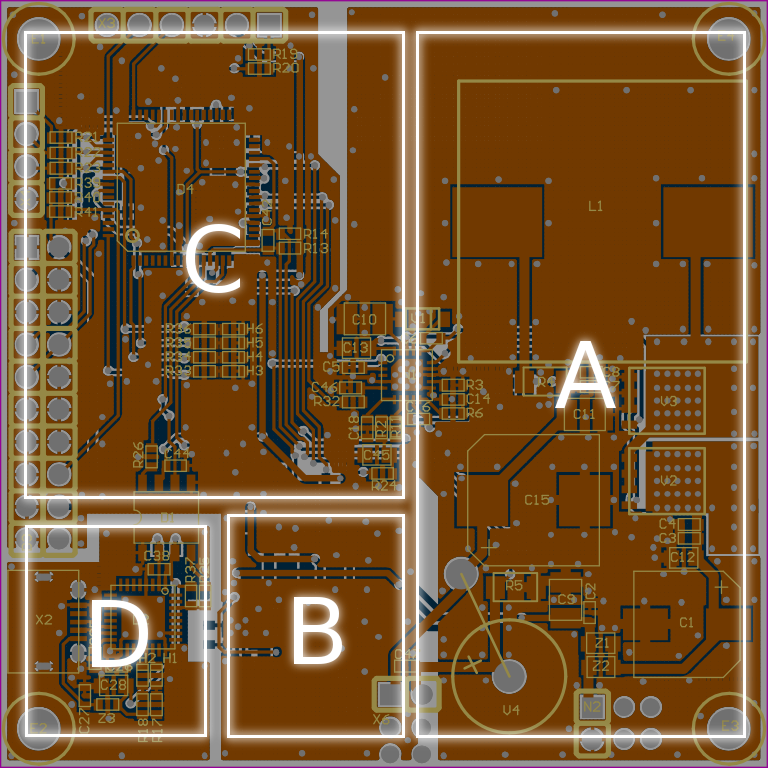
\includegraphics[width=.45\linewidth]{images/pcb/partitioning.png}
    \caption{Partitioning scheme of component groups.
        \textbf{A:} High power components
        \textbf{B:} Voltage rails
        \textbf{C:} Digital logic
        \textbf{D:} Isolated transceiver logic
    }
    \label{fig:pcb:partitioning}
\end{figure}

\begin{figure}[th!]
    \centering
    \begin{minipage}{.4\textwidth}
        \centering
        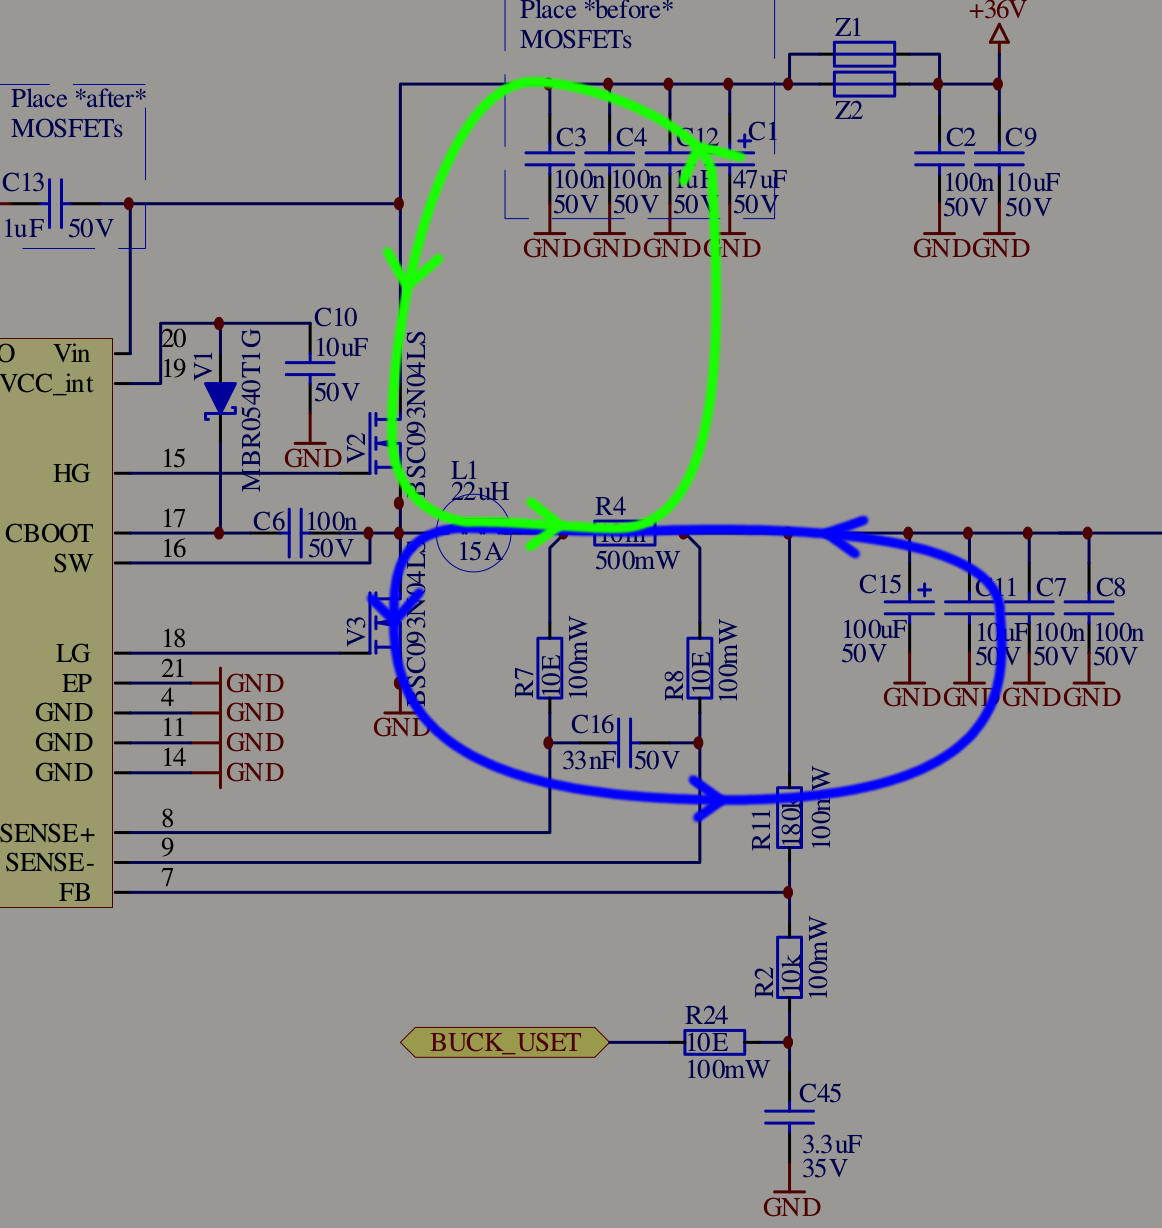
\includegraphics[width=\textwidth]{images/circuit/schematic_high_current.png}
        \caption{Critical high current, high frequency loops in the schematic}
    \end{minipage}
    \begin{minipage}{.5\textwidth}
        \centering
        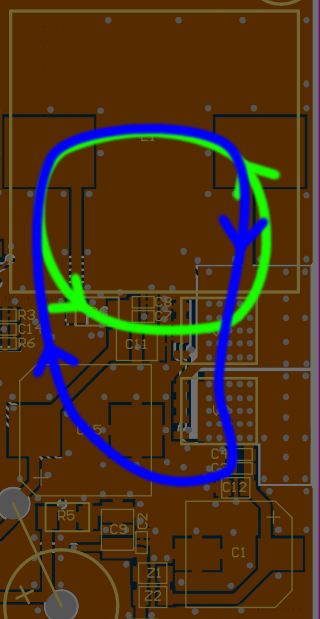
\includegraphics[width=.6\textwidth]{images/pcb/buck2.png}
        \caption{High current, high frequency loops are routed as tightly as possible}
    \end{minipage}
\end{figure}

